\chapter{Advanced Methods}\label{adv_meth}

\section{Overview}\label{adv_meth:overview}

A variety of ``meta-algorithm'' capabilities have been developed in 
order to provide a mechanism for employing individual iterators and 
models as reusable components within higher-level solution approaches. 
%It was driven by the observed need for ``meta-optimization'' and other 
%high level systems analysis procedures in real-world engineering 
%design problems. 
This capability allows the use of existing iterative algorithm and
computational model software components as building blocks to
accomplish more sophisticated studies, such as hybrid,
multistart, Pareto, or surrogate-based minimization.  Further
multi-component capabilities are enabled by the model recursion
capabilities described in Chapter~\ref{models} with specific examples
in Chapter~\ref{adv_models}.
%When these model recursion specifications are sufficient to completely
%describe a multi-iterator, multi-model solution approach, then a
%separate meta-iterator specification is not used (see
%Chapter~\ref{adv_models} for examples).

\section{Hybrid Minimization}\label{adv_meth:hybrid}

In the hybrid minimization method (keyword: \texttt{hybrid}), a
sequence of minimization methods are applied to find an optimal design
point. The goal of this method is to exploit the strengths of
different minimization algorithms through different stages of the
minimization process. Global/local optimization hybrids (e.g., genetic
algorithms combined with nonlinear programming) are a common example
in which the desire for a global optimum is balanced with the need for
efficient navigation to a local optimum. An important related feature
is that the sequence of minimization algorithms can employ models of
varying fidelity. In the global/local case, for example, it would
often be advantageous to use a low-fidelity model in the global search
phase, followed by use of a more refined model in the local search
phase.

The specification for hybrid minimization involves a list of
method identifier strings, and each of the corresponding method
specifications has the responsibility for identifying the model
specification (which may in turn identify variables, interface, and
responses specifications) that each method will use (see the Dakota
Reference Manual~\cite{RefMan} and the example discussed below).
Currently, only the sequential hybrid approach is available. The
\texttt{embedded} and \texttt{collaborative} approaches are
not fully functional at this time.

In the \texttt{sequential} hybrid minimization approach, a sequence
of minimization methods is invoked in the order specified in the
Dakota input file. After each method completes execution, 
the best solution or solutions from that method are used as the
starting point(s) for the following method. 
The number of solutions transferred 
is defined by how many that method can generate and how many the 
user specifies with the individual method keyword \texttt{final\_solutions}. 
For example, currently only a few of the global optimization methods such as 
genetic algorithms (e.g. \texttt{moga} and \texttt{coliny\_ea}) and 
sampling methods return multiple solutions.  In this case, 
the specified number of solutions from the previous 
method will be used to initialize the subsequent method.  If the subsequent 
method cannot accept multiple input points (currently only a few methods 
such as the genetic algorithms in JEGA allow multiple input points), then 
multiple instances of the subsequent method are generated, each one 
initialized by one of the optimal solutions from the previous method. 
For example, if LHS sampling were run as the first method and 
the number of final solutions was 10 and the DOT conjugate gradient 
was the second method, there would be 10 instances of \texttt{dot\_frcg} 
started, each with a separate LHS sample solution as its initial point. 
Method switching is governed
by the separate convergence controls of each method; that is,
\emph{each method is allowed to run to its own internal definition of
completion without interference}. Individual method completion may be
determined by convergence criteria (e.g.,
\texttt{convergence\_tolerance}) or iteration limits (e.g.,
\texttt{max\_iterations}).  

%The \texttt{adaptive} option
%is similar, with the difference that the progress of each method is
%monitored and method switching is enforced according to
%externally-defined relative progress metrics.  

%The \texttt{embedded} approach is restricted to special tightly-coupled
%hybrid algorithms in which local searches are used periodically to
%accelerate a global search.  These hybrids do not contain a discrete
%method switch, but rather repeatedly apply a local algorithm within
%the context of the global algorithm.

Figure~\ref{adv_meth:figure01} shows a Dakota input file that specifies
a sequential hybrid optimization method to solve the
``textbook'' optimization test problem.
The \path{textbook_hybrid_strat.in} file
provided in \path{dakota/share/dakota/examples/users} starts with a
\dakotakw{coliny_ea} solution which feeds its best point into a
\dakotakw{coliny_pattern_search} optimization which feeds its best
point into \dakotakw{optpp_newton}. While this approach is overkill for
such a simple problem, it is useful for demonstrating the coordination
between multiple sub-methods in the hybrid minimization algorithm.

The three optimization methods are identified using the
\texttt{method\_list} specification in the hybrid method section of the
input file. The identifier strings listed in the specification are
`\texttt{GA}' for genetic algorithm, `\texttt{PS}' for pattern search,
and `\texttt{NLP}' for nonlinear programming. Following the hybrid method
keyword block are the three corresponding method keyword blocks. Note
that each method has a tag following the \texttt{id\_method} keyword
that corresponds to one of the method names listed in the hybrid method
keyword block. By following the identifier tags from \texttt{method}
to \texttt{model} and from \texttt{model} to \texttt{variables},
\texttt{interface}, and \texttt{responses}, it is easy to see the
specification linkages for this problem. The GA optimizer runs first
and uses model `\texttt{M1}' which includes variables `\texttt{V1}',
interface `\texttt{I1}', and responses `\texttt{R1}'. 
Note that in the specification, \texttt{final\_solutions=1}, 
so only one (the best) solution is returned from the GA.  
However, it is possible to change this to \texttt{final\_solutions=5}
and get five solutions passed from the GA to the Pattern Search
(for example).  Once the GA is complete, the PS optimizer starts from the 
best GA result and again
uses model `\texttt{M1}'. Since both GA and PS are nongradient-based
optimization methods, there is no need for gradient or Hessian
information in the `\texttt{R1}' response keyword block. The NLP
optimizer runs last, using the best result from the PS method as its
starting point.  It uses model `\texttt{M2}' which includes the same
`\texttt{V1}' and `\texttt{I1}' keyword blocks, but uses the responses
keyword block `\texttt{R2}' since the full Newton optimizer used in
this example (\texttt{optpp\_newton}) needs analytic gradient and
Hessian data to perform its search.
\begin{figure}
  \centering
  \begin{bigbox}
    \begin{tiny}
      \verbatimtabinput[8]{../../test/examples-users/textbook_hybrid_strat.in}
    \end{tiny}
  \end{bigbox}
  \caption{Dakota input file for a sequential hybrid optimization method --
see \protect\path{dakota/share/dakota/examples/users/textbook_hybrid_strat.in} }
  \label{adv_meth:figure01}
\end{figure}

\section{Multistart Local Minimization}\label{adv_meth:multistart}

A simple, heuristic, global minimization technique is to use many
local minimization runs, each of which is started from a different
initial point in the parameter space. This is known as multistart
local minimization. This is an attractive method in situations where
multiple local optima are known or expected to exist in the parameter
space. However, there is no theoretical guarantee that the global
optimum will be found. This approach combines the efficiency of local
minimization methods with a user-specified global stratification
(using a specified \texttt{starting\_points} list, a number of
specified \texttt{random\_starts}, or both; see the Dakota Reference
Manual~\cite{RefMan} for additional specification details). Since
solutions for different starting points are independent, parallel
computing may be used to concurrently run the local minimizations.

An example input file for multistart local optimization on the
``quasi\_sine'' test function (see \path{quasi_sine_fcn.C} in
\path{dakota_source/test}) is shown in Figure~\ref{adv_meth:figure02}.
The method keyword block in the input file contains the keyword
\texttt{multi\_start}, along with the set of starting points (3 random 
and 5 listed) that will be used for the optimization runs. The other
keyword blocks in the input file are similar to what would be used in
a single optimization run.

\begin{figure}
  \centering
  \begin{bigbox}
    \begin{small}
      \verbatimtabinput[8]{../../test/examples-users/qsf_multistart_strat.in}
    \end{small}
  \end{bigbox}
  \caption{Dakota input file for a multistart local optimization method --
see \protect\path{dakota/share/dakota/examples/users/qsf_multistart_strat.in} }
  \label{adv_meth:figure02}
\end{figure}

The \texttt{quasi\_sine} test function has multiple local minima, but
there is an overall trend in the function that tends toward the global
minimum at $(x1,x2)=(0.177,0.177)$. See~\cite{Giu00} for more
information on this test function. Figure~\ref{adv_meth:figure03} shows
the results summary for the eight local optimizations performed. From
the five specified starting points and the 3 random starting points
(as identified by the \texttt{x1}, \texttt{x2} headers), the eight
local optima (as identified by the \texttt{x1*},
\texttt{x2*} headers) are all different and only one of the local
optimizations finds the global minimum.

\begin{figure}
\centering
\begin{bigbox}
\begin{footnotesize}
\begin{verbatim}
<<<<< Results summary:
   set_id             x1             x2            x1*            x2*         obj_fn 
        1           -0.8           -0.8  -0.8543728666  -0.8543728666   0.5584096919 
        2           -0.8            0.8  -0.9998398719    0.177092822    0.291406596 
        3            0.8           -0.8    0.177092822  -0.9998398719    0.291406596 
        4            0.8            0.8   0.1770928217   0.1770928217   0.0602471946 
        5              0              0  0.03572926375  0.03572926375  0.08730499239 
        6  -0.7767971993  0.01810943539  -0.7024118387  0.03572951143   0.3165522387 
        7  -0.3291571008  -0.7697378755   0.3167607374  -0.4009188363   0.2471403213 
        8   0.8704730469   0.7720679005    0.177092899   0.3167611757  0.08256082751 
\end{verbatim}
\end{footnotesize}
\end{bigbox}
\caption{Dakota results summary for a multistart local optimization method.}
\label{adv_meth:figure03}
\end{figure}

\section{Pareto Optimization}\label{adv_meth:pareto}

The Pareto optimization method (keyword: \dakotakw{pareto_set}) is
one of three multiobjective optimization capabilities discussed in
Section~\ref{opt:additional:multiobjective}. In the Pareto
optimization method, multiple sets of multiobjective weightings are
evaluated. The user can specify these weighting sets in the method
keyword block using a \dakotakw{multi_objective_weight_sets} list, a
number of \dakotakw{random_weight_sets}, or both (see the Dakota
Reference Manual~\cite{RefMan} for additional specification details).

Dakota performs one multiobjective optimization problem for each set
of multiobjective weights. The collection of computed optimal
solutions form a Pareto set, which can be useful in making trade-off
decisions in engineering design. Since solutions for different
multiobjective weights are independent, parallel computing may be used
to concurrently execute the multiobjective optimization problems.

Figure~\ref{adv_meth:figure05} shows the results summary for the
Pareto-set optimization method. For the four multiobjective
weighting sets (as identified by the \texttt{w1}, \texttt{w2},
\texttt{w3} headers), the local optima (as identified by the
\texttt{x1}, \texttt{x2} headers) are all different and correspond to
individual objective function values of ($f_1,f_2,f_3$) =
(0.0,0.5,0.5), (13.1,-1.2,8.16), (532.,33.6,-2.9), and (0.125,0.0,0.0)
(note: the composite objective function is tabulated under the
\texttt{obj\_fn} header).  The first three solutions reflect exclusive
optimization of each of the individual objective functions in turn,
whereas the final solution reflects a balanced weighting and the
lowest sum of the three objectives.  Plotting these ($f_1,f_2,f_3$)
triplets on a 3-dimensional plot results in a Pareto surface (not
shown), which is useful for visualizing the trade-offs in the
competing objectives.

\begin{figure}
  \centering
  \begin{bigbox}
    \begin{small}
      \verbatimtabinput[8]{../../test/examples-users/textbook_pareto_strat.in}
    \end{small}
  \end{bigbox}
  \caption{Dakota input file for the Pareto optimization method --
see \protect\path{dakota/share/dakota/examples/users/textbook_pareto_strat.in} }
  \label{adv_meth:figure04}
\end{figure}

\begin{figure}
\centering
\begin{bigbox}
\begin{scriptsize}
\begin{verbatim}
<<<<< Results summary:
   set_id             w1             w2             w3             x1             x2         obj_fn
        1              1              0              0   0.9996554048    0.997046351 7.612301561e-11
        2              0              1              0            0.5            2.9           -1.2
        3              0              0              1            5.8 1.12747589e-11           -2.9
        4          0.333          0.333          0.333            0.5   0.5000000041       0.041625
\end{verbatim}
\end{scriptsize}
\end{bigbox}
\caption{Dakota results summary for the Pareto-set optimization
  method.}
\label{adv_meth:figure05}
\end{figure}

\section{Mixed Integer Nonlinear Programming (MINLP)}\label{adv_meth:minlp}

Many nonlinear optimization problems involve a combination of discrete
and continuous variables. These are known as mixed integer nonlinear
programming (MINLP) problems. A typical MINLP optimization problem is
formulated as follows:

\begin{eqnarray}
  \hbox{minimize:} & & f(\mathbf{x,d})\nonumber\\
  \hbox{subject to:} & & \mathbf{g}_{L} \leq \mathbf{g(x,d)}
    \leq \mathbf{g}_{U}\nonumber\\
  & & \mathbf{h(x,d)}=\mathbf{h}_{t}\label{adv_meth:equation01}\\
  & & \mathbf{x}_{L} \leq \mathbf{x} \leq \mathbf{x}_{U}\nonumber\\
  & & \mathbf{d} \in \{-2,-1,0,1,2\}\nonumber
\end{eqnarray}

where $\mathbf{d}$ is a vector whose elements are integer values. In
situations where the discrete variables can be temporarily relaxed
(i.e., noncategorical discrete variables, see
Section~\ref{variables:design:ddv}), the branch-and-bound algorithm
can be applied. Categorical variables (e.g., true/false variables,
feature counts, etc.) that are not relaxable cannot be used with the
branch and bound method.  During the branch and bound process, the
discrete variables are treated as continuous variables and the
integrality conditions on these variables are incrementally enforced
through a sequence of optimization subproblems.  By the end of this
process, an optimal solution that is feasible with respect to the
integrality conditions is computed.

Dakota's branch and bound method (keyword:
\texttt{branch\_and\_bound}) can solve optimization problems having
either discrete or mixed continuous/discrete variables. This method
uses the parallel branch-and-bound algorithm from the PEBBL software
%package~\cite{Eck97,Eck01} to generate a series of optimization
package~\cite{Eck09} to generate a series of optimization
subproblems (``branches''). These subproblems are solved as continuous
variable problems using any of Dakota's nonlinear optimization
algorithms (e.g., DOT, NPSOL). When a solution to a branch is feasible
with respect to the integrality constraints, it provides an upper
bound on the optimal objective function, which can be used to prune
branches with higher objective functions that are not yet
feasible. Since solutions for different branches are independent,
parallel computing may be used to concurrently execute the
optimization subproblems.

PEBBL, by itself, targets the solution of mixed integer linear
programming (MILP) problems, and through coupling with Dakota's
nonlinear optimizers, is extended to solution of MINLP problems. In
the case of MILP problems, the upper bound obtained with a feasible
solution is an exact bound and the branch and bound process is
provably convergent to the global minimum. For nonlinear problems
which may exhibit nonconvexity or multimodality, the process is
heuristic in general, since there may be good solutions that are
missed during the solution of a particular branch. However, the
process still computes a series of locally optimal solutions, and is
therefore a natural extension of the results from local optimization
techniques for continuous domains. Only with rigorous global
optimization of each branch can a global minimum be guaranteed when
performing branch and bound on nonlinear problems of unknown
structure.

In cases where there are only a few discrete variables and when the
discrete values are drawn from a small set, then it may be reasonable
to perform a separate optimization problem for all of the possible
combinations of the discrete variables. However, this brute force
approach becomes computationally intractable if these conditions are
not met. The branch-and-bound algorithm will generally require
solution of fewer subproblems than the brute force method, although it
will still be significantly more expensive than solving a purely
continuous design problem.

\subsection{Example MINLP Problem}\label{adv_meth:minlp:example}

As an example, consider the following MINLP problem~\cite{Eld99}:

\begin{eqnarray}
  \hbox{minimize:} & &
  f(\mathbf{x})=\sum_{i=1}^{6}(x_{i}-1.4)^{4}\nonumber\\
  & & g_{1}=x_{1}^{2}-\frac{x_{2}}{2} \leq 0\nonumber\\
  & & g_{2}=x_{2}^{2}-\frac{x_{1}}{2} \leq 0\label{adv_meth:equation02}\\
  & & -10 \leq x_{1},x_{2},x_{3},x_{4} \leq 10\nonumber\\
  & & x_{5},x_{6} \in \{0,1,2,3,4\}\nonumber
\end{eqnarray}

This problem is a variant of the textbook test problem described in
Section~\ref{additional:textbook}. In addition to the introduction of
two integer variables, a modified value of $1.4$ is used inside the
quartic sum to render the continuous solution a non-integral solution.
%Figure~\ref{adv_meth:figure06} shows a Dakota input file for solving this
%problem. This input file is named \path{dakota_bandb.in} in the
%\path{dakota/share/dakota/test} directory. Note the specification for the
%discrete variables, where lower and upper bounds are given. The
%discrete variables can take on any integer value within these bounds.

%\begin{figure}
%  \centering
%  \begin{bigbox}
%    \begin{small}
%      \verbatimtabinput[8]{../../test/examples-users/dakota_bandb.in}
%    \end{small}
%  \end{bigbox}
%  \caption{Dakota input file for the branch-and-bound method for
%    solving MINLP optimization problems.}
%  \label{adv_meth:figure06}
%\end{figure}

Figure~\ref{adv_meth:figure07} shows the sequence of branches generated
for this problem.  The first optimization subproblem relaxes the
integrality constraint on parameters $x_{5}$ and $x_{6}$, so that $0
\leq x_{5} \leq 4$ and $0 \leq x_{6} \leq 4$. The values for $x_{5}$
and $x_{6}$ at the solution to this first subproblem are
$x_{5}=x_{6}=1.4$.  Since $x_{5}$ and $x_{6}$ must be integers, the
next step in the solution process ``branches'' on parameter $x_{5}$ to
create two new optimization subproblems; one with $0 \leq x_{5} \leq
1$ and the other with $2 \leq x_{5} \leq 4$.  Note that, at this first
branching, the bounds on $x_{6}$ are still $0 \leq x_{6} \leq 4$.
Next, the two new optimization subproblems are solved.  Since they are
independent, they can be performed in parallel.  The branch-and-bound
process continues, operating on both $x_{5}$ and $x_{6}$ , until a
optimization subproblem is solved where $x_{5}$ and $x_{6}$ are
integer-valued. At the solution to this problem, the optimal values
for $x_{5}$ and $x_{6}$ are $x_{5}=x_{6}=1$.

\begin{figure}
  \centering
  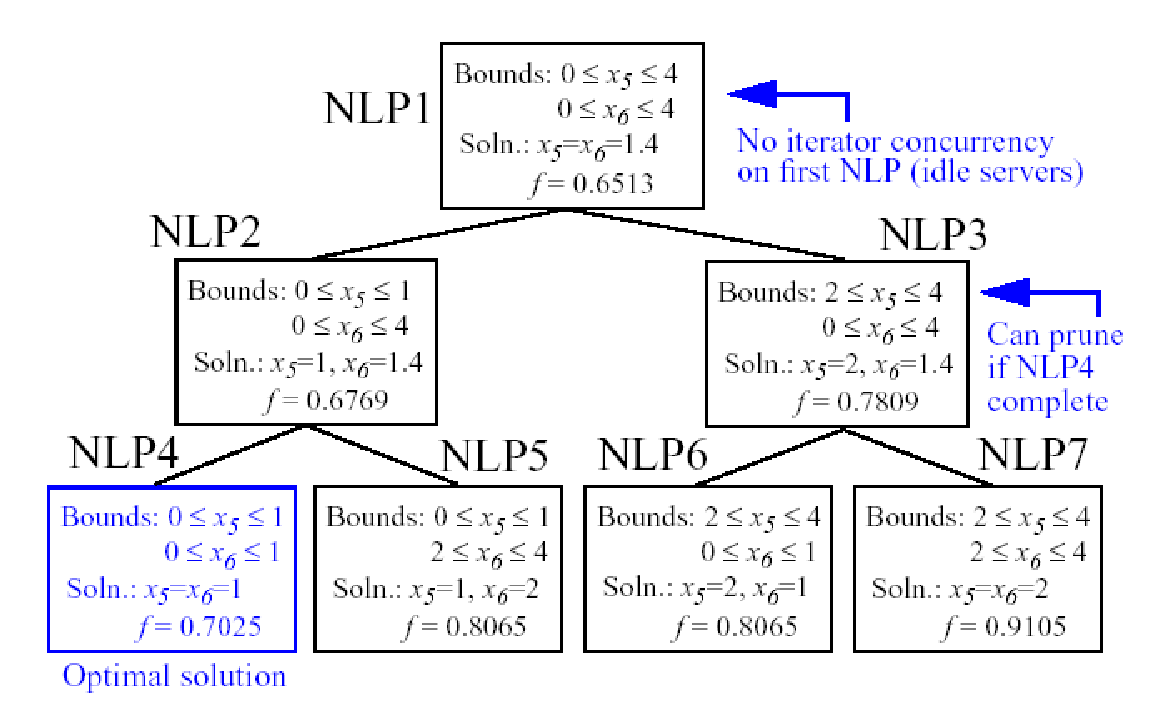
\includegraphics[scale=0.75]{images/branch_history}
  \caption{Branching history for example MINLP optimization problem.}
  \label{adv_meth:figure07}
\end{figure}

In this example problem, the branch-and-bound algorithm executes as
few as five and no more than seven optimization subproblems to reach
the solution. For comparison, the brute force approach would require
25 optimization problems to be solved (i.e., five possible values for
each of $x_{5}$ and $x_{6}$ ).

In the example given above, the discrete variables are integer-valued.
In some cases, the discrete variables may be real-valued, such as $x
\in \{0.0,0.5,1.0,1.5,2.0\}$.  The branch-and-bound algorithm is
restricted to work with integer values. Therefore, it is up to the
user to perform a transformation between the discrete integer values
from Dakota and the discrete real values that are passed to the
simulation code (see Section~\ref{variables:design:ddv}).  When
integrality is not being relaxed, a common mapping is to use the
integer value from Dakota as the index into a vector of discrete real
values.  However, when integrality is relaxed, additional logic for
interpolating between the discrete real values is needed.
% Note: it should be straightforward to extend MINLP to support
% general discrete variables, if PICO would support it.  Does this
% come up in MILP for logistics, etc.?

\section{Surrogate-Based Minimization}\label{adv_meth:sbm}

Surrogate models approximate an original, high fidelity ``truth''
model, typically at reduced computational cost.  In Dakota, several
surrogate model selections are possible, which are categorized as data
fits, multifidelity models, and reduced-order models, as described in
Section~\ref{models:surrogate}.  In the context of minimization
(optimization or calibration), surrogate models can speed convergence
by reducing function evaluation cost or smoothing noisy response
functions.  Three categories of surrogate-based minimization are
discussed in this chapter:
\begin{itemize}
\item Trust region-managed surrogate-based local minimization, with
  data fit surrogate, multifidelity models, or reduced-order models.

\item Surrogate-based global minimization, where a single surrogate is
  built (and optionally iteratively updated) over the whole design
  space.

\item Efficient global minimization: nongradient-based constrained and
  unconstrained optimization and nonlinear least squares based on
  Gaussian process models, guided by an expected improvement function.
\end{itemize}

\subsection{Surrogate-Based Local Minimization}\label{adv_meth:sbm:sblm}

In the surrogate-based local minimization method (keyword:
\texttt{surrogate\_based\_local}) the minimization algorithm operates
on a surrogate model instead of directly operating on the
computationally expensive simulation model. The surrogate model can be
based on data fits, multifidelity models, or reduced-order models, as
described in Section~\ref{models:surrogate}. Since the surrogate will
generally have a limited range of accuracy, the surrogate-based local
algorithm periodically checks the accuracy of the surrogate model
against the original simulation model and adaptively manages the
extent of the approximate optimization cycles using a trust region
approach.

%The surrogate-based local method in
%Dakota can be implemented using heuristic rules (less expensive) or
%provably-convergent rules (more expensive). The heuristic approach
%is particularly effective on real-world engineering design problems
%that contain nonsmooth features (e.g., slope discontinuities,
%numerical noise) where gradient-based optimization methods often have
%trouble, and where the computational expense of the simulation
%precludes the use of nongradient-based methods.

Refer to the Dakota Theory Manual~\cite{TheoMan} for algorithmic
details on iterate acceptance, merit function formulations,
convergence assessment, and constraint relaxation.


\subsubsection{SBO with Data Fits}\label{adv_meth:sbm:sblm:surface}

When performing SBO with local, multipoint, and global data fit
surrogates, it is necessary to regenerate or update the data fit for
each new trust region.  In the global data fit case, this can mean
performing a new design of experiments on the original high-fidelity
model for each trust region, which can effectively limit the approach
to use on problems with, at most, tens of variables.
Figure~\ref{fig:sbo_df} displays this case.  However, an important
benefit of the global sampling is that the global data fits can tame
poorly-behaved, nonsmooth, discontinuous response variations within
the original model into smooth, differentiable, easily navigated
surrogates.  This allows SBO with global data fits to extract the
relevant global design trends from noisy simulation data.

\begin{figure}
  \centering
  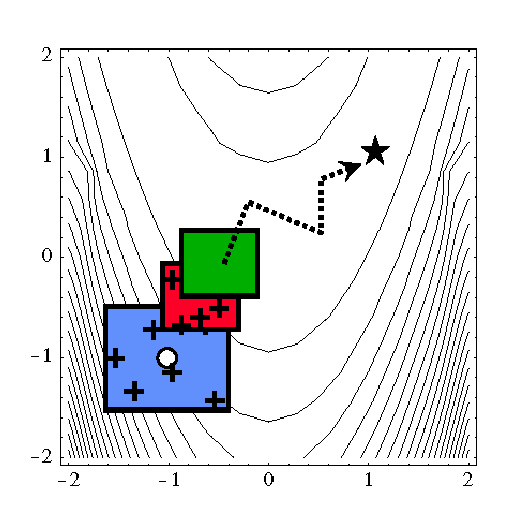
\includegraphics[width=.4\textwidth]{images/sbo_df}
  \caption{SBO iteration progression for global data fits.}
  \label{fig:sbo_df}
\end{figure}
When enforcing local consistency between a global data fit surrogate
and a high-fidelity model at a point, care must be taken to balance
this local consistency requirement with the global accuracy of the
surrogate.  In particular, performing a correction on an existing
global data fit in order to enforce local consistency can skew the
data fit and destroy its global accuracy.  One approach for achieving
this balance is to include the consistency requirement within the data
fit process by constraining the global data fit calculation (e.g.,
using constrained linear least squares).  This allows the data fit to
satisfy the consistency requirement while still addressing global
accuracy with its remaining degrees of freedom.
% Use figure from Theresa's paper?  Use equations from notes?
Embedding the consistency within the data fit also reduces the
sampling requirements.  For example, a quadratic polynomial normally
requires at least $(n+1)(n+2)/2$ samples for $n$ variables to perform
the fit.  However, with an embedded first-order consistency constraint
at a single point, the minimum number of samples is reduced by $n+1$ 
to $(n^2+n)/2$.
% With gradient information in each sample, this can be further
% reduced to ceil(n+2/2) samples.
%This corresponds to defining the terms of a symmetric Hessian matrix
%and points to an alternate approach.  Rather than enforcing
%consistency through constrained least squares, one can embed
%consistency directly by employing a Taylor series centered at the
%point of local consistency enforcement and globally estimating the
%higher order terms.  In the quadratic polynomial example, a
%second-order Taylor series with globally estimated Hessian terms
%requires the same $(n^2+n)/2$ samples and directly satisfies
%first-order consistency.  To further reduce sampling requirements in
%this case, one can choose to perform only partial updates (e.g., the
%diagonal) of the Hessian matrix~\cite{Per02}.

% Additional research area: Exploiting variance estimators to guide
% global search (e.g., kriging)

In the local and multipoint data fit cases, the iteration progression
will appear as in Fig.~\ref{fig:sbo_mh}.  Both cases involve a single
new evaluation of the original high-fidelity model per trust region,
with the distinction that multipoint approximations reuse information
from previous SBO iterates.  Like model hierarchy surrogates, these
techniques scale to larger numbers of design variables.  Unlike model
hierarchy surrogates, they generally do not require surrogate
corrections, since the matching conditions are embedded in the
surrogate form (as discussed for the global Taylor series approach
above).  The primary disadvantage to these surrogates is that the
region of accuracy tends to be smaller than for global data fits and
multifidelity surrogates, requiring more SBO cycles with smaller trust
regions.
%In SBO with surface fit functions, a sequence of optimization
%subproblems are evaluated, each of which is confined to a subset of
%the parameter space known as a ``trust region.'' Inside each trust
%region, Dakota's data sampling methods are used to evaluate the
%response quantities at a small number (order $10^{1}$ to $10^{2}$) of
%design points. Next, multidimensional surface fitting is performed to
%create a surrogate function for each of the response quantities.
%Finally, optimization is performed using the surrogate functions in
%lieu of the actual response quantities, and the optimizer's search is
%limited to the region inside the trust region bounds. A validation
%procedure is then applied to compare the predicted improvement in the
%response quantities to the actual improvement in the response
%quantities. Based on the results of this validation, the optimum
%design point is either accepted or rejected and the size of the trust
%region is either expanded, contracted, or left unchanged. The sequence
%of optimization subproblems continues until the SBO convergence 
%criteria are satisfied
More information on the design of experiments methods is available in
Chapter~\ref{dace}, and the data fit surrogates are described in
Section~\ref{models:surrogate:datafit}.

Figure~\ref{sbm:sblm_rosen} shows a Dakota input file that implements
surrogate-based optimization on Rosenbrock's function.
The first method keyword block contains the SBO 
keyword \texttt{surrogate\_based\_local}, plus the commands for
specifying the trust region size and scaling factors. The optimization
portion of SBO, using the CONMIN Fletcher-Reeves conjugate gradient method,
is specified in the following keyword blocks for
\texttt{method}, \texttt{model}, \texttt{variables}, and
\texttt{responses}.  The model used by the optimization method 
specifies that a global surrogate will be used to map variables into
responses (no \texttt{interface} specification is used by the
surrogate model). The global surrogate is constructed using a DACE
method which is identified with the \texttt{`SAMPLING'} identifier.
This data sampling portion of SBO is specified in the final set of
keyword blocks for \texttt{method}, \texttt{model},
\texttt{interface}, and \texttt{responses} (the earlier 
\texttt{variables} specification is reused). This example problem uses 
the Latin hypercube sampling method in the LHS software to select 10
design points in each trust region. A single surrogate model is
constructed for the objective function using a quadratic polynomial.
The initial trust region is centered at the design point
$(x_1,x_2)=(-1.2,1.0)$, and extends $\pm 0.4$ (10\% of the global
bounds) from this point in the $x_1$ and $x_2$ coordinate directions.
\begin{figure}
  \begin{bigbox}
    \begin{tiny}
      \verbatimtabinput[8]{../../test/examples-users/rosen_opt_sbo.in}
    \end{tiny}
  \end{bigbox}
  \caption{Dakota input file for the surrogate-based local optimization
    example --
see \protect\path{dakota/share/dakota/examples/users/rosen_opt_sbo.in} }
  \label{sbm:sblm_rosen}
\end{figure}

If this input file is executed in Dakota, it will converge to the
optimal design point at $(x_{1},x_{2})=(1,1)$ in approximately 800
function evaluations. While this solution is correct, it is obtained
at a much higher cost than a traditional gradient-based optimizer
(e.g., see the results obtained in Section~\ref{tutorial:examples:optimization}).
This demonstrates that the SBO method with global data fits is not
really intended for use with smooth continuous optimization problems;
direct gradient-based optimization can be more efficient for such
applications. Rather, SBO with global data fits is best-suited for the
types of problems that occur in engineering design where the response
quantities may be discontinuous, nonsmooth, or may have multiple local
optima~\cite{Giu02}. In these types of engineering design problems,
traditional gradient-based optimizers often are ineffective, whereas
global data fits can extract the global trends of interest despite the
presence of local nonsmoothness (for an example problem with multiple
local optima, look in \path{dakota/share/dakota/test} for the file
\path{dakota_sbo_sine_fcn.in}~\cite{Giu00}).

The surrogate-based local minimizer is only mathematically
guaranteed to find a local minimum. However, in practice, SBO can often find 
the global minimum.  Due to the random sampling method used within the
SBO algorithm, the SBO method will solve a given problem a little differently 
each time it is run (unless the user specifies a particular random
number seed in the dakota input file as is shown in Figure~\ref{sbm:sblm_rosen}). 
Our experience on the quasi-sine function mentioned above is that if 
you run this problem 10 times with the same starting conditions but different 
seeds, then you will find the global minimum in about 70-80\% of the trials.
This is good performance for what is mathematically only a local optimization method.

\subsubsection{SBO with Multifidelity Models}\label{adv_meth:sbm:sblm:multifidelity}

When performing SBO with model hierarchies, the low-fidelity model is
normally fixed, requiring only a single high-fidelity evaluation to
compute a new correction for each new trust region.
Figure~\ref{fig:sbo_mh} displays this case.  This renders the
multifidelity SBO technique more scalable to larger numbers of design
variables since the number of high-fidelity evaluations per iteration
(assuming no finite differencing for derivatives) is independent of
the scale of the design problem.  However, the ability to smooth
poorly-behaved response variations in the high-fidelity model is lost,
and the technique becomes dependent on having a well-behaved
low-fidelity model\footnote{It is also possible to use a hybrid data
fit/multifidelity approach in which a smooth data fit of a noisy low
fidelity model is used in combination with a high fidelity model}.  In
addition, the parameterizations for the low and high-fidelity models
may differ, requiring the use of a mapping between these
parameterizations.  Space mapping, corrected space mapping, POD
mapping, and hybrid POD space mapping are being explored for this
purpose~\cite{Rob06a,Rob06b}.

\begin{wrapfigure}{r}{.3\textwidth}
  \centering
  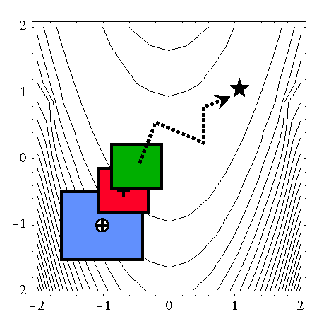
\includegraphics[width=.3\textwidth]{images/sbo_mh}
  \caption{SBO iteration progression for model hierarchies.}
  \label{fig:sbo_mh}
\end{wrapfigure}
%\begin{figure}
%\epsfxsize 3in
%\centerline{\epsfbox{sbo_mh.eps}}
%\caption{SBO iteration progression for model hierarchies.}
%\label{fig:sbo_mh}
%\end{figure}

When applying corrections to the low-fidelity model, there is no
concern for balancing global accuracy with the local consistency
requirements.  However, with only a single high-fidelity model evaluation
at the center of each trust region, it is critical to use the best
correction possible on the low-fidelity model in order to achieve
rapid convergence rates to the optimum of the high-fidelity
model~\cite{Eld04}.

%SBO can also be applied with multifidelity, or hierarchical, models,
%i.e., where one has available both a high-fidelity computational model
%and a low-fidelity computational model. This situation can occur when
%the low-fidelity model neglects some physical phenomena (e.g.,
%viscosity, heat transfer, etc.) that are included in the high-fidelity
%model, or when the low-fidelity model has a lower resolution
%computational mesh than the high-fidelity model. In many cases, the
%low-fidelity model can serve as a surrogate for the high-fidelity
%model during the optimization process. Thus, the low-fidelity model
%can be used in SBO in a manner similar to the use of surface fit models
%described in Section~\ref{adv_meth:sbm:sblm:surface}. A key difference
%in SBO with hierarchical surrogates is that a design of experiments
%using the high-fidelity model is not required; rather high-fidelity
%evaluations are only needed at the center of the current trust-region
%and the predicted optimum point in order to correct the low-fidelity
%model and verify improvement, respectively. Another difference is that
%one of the four types of correction described in
%Section~\ref{adv_meth:sbm:sblm:surface} is required for SBO with 
%multifidelity models.

A multifidelity test problem named
\path{dakota_sbo_hierarchical.in} is available in
\path{dakota/share/dakota/test} to demonstrate this SBO approach. This test
problem uses the Rosenbrock function as the high fidelity model and a
function named ``lf\_rosenbrock'' as the low fidelity model. Here,
lf\_rosenbrock is a variant of the Rosenbrock function (see
\path{dakota_source/test/lf_rosenbrock.C} for formulation) with the
minimum point at $(x_1,x_2)=(0.80,0.44)$, whereas the minimum of the
original Rosenbrock function is $(x_1,x_2)=(1,1)$. Multifidelity SBO
locates the high-fidelity minimum in 11 high fidelity evaluations for
additive second-order corrections and in 208 high fidelity evaluations
for additive first-order corrections, but fails for zeroth-order
additive corrections by converging to the low-fidelity minimum.

\subsubsection{SBO with Reduced Order Models}\label{adv_meth:sbm:sblm:rom}

When performing SBO with reduced-order models (ROMs), the ROM is
mathematically generated from the high-fidelity model.  A critical
issue in this ROM generation is the ability to capture the effect of
parametric changes within the ROM.  Two approaches to parametric ROM
are extended ROM (E-ROM) and spanning ROM (S-ROM)
techniques~\cite{Wei06}.  Closely related techniques include tensor
singular value decomposition (SVD) methods~\cite{Lat00}.  In the
single-point and multipoint E-ROM cases, the SBO iteration can appear
as in Fig.~\ref{fig:sbo_mh}, whereas in the S-ROM, global E-ROM, and
tensor SVD cases, the SBO iteration will appear as in
Fig.~\ref{fig:sbo_df}.  In addition to the high-fidelity model
analysis requirements, procedures for updating the system matrices and
basis vectors are also required.

Relative to data fits and multifidelity models, ROMs have some
attractive advantages.  Compared to data fits such as regression-based
polynomial models, they are more physics-based and would be expected
to be more predictive (e.g., in extrapolating away from the immediate
data).  Compared to multifidelity models, ROMS may be more practical
in that they do not require multiple computational models or meshes
which are not always available.  The primary disadvantage is potential
invasiveness to the simulation code for projecting the system using
the reduced basis.


\subsection{Surrogate-Based Global Minimization}\label{adv_meth:sbm:sbgm}

In surrogate-based global minimization, the optimization method
operates over the whole domain on a global surrogate constructed over
a (static or adaptively augmented) set of truth model sample
points. There are no trust regions and no convergence guarantees for
the original optimization problem, though optimizers can be reasonably
expected to converge as expected on the approximate (surrogate)
problem.

In the first, and perhaps most common, global surrogate use case, a
user wishes to use existing function evaluations or a fixed sample
size (perhaps based on computational cost and allocation of resources)
to build a surrogate once and optimize on it.  For this single global
optimization on a surrogate model), the set of surrogate build points
is determined in advance. Contrast this with trust-region local
methods in which the number of ``true'' function evaluations depends
on the location and size of the trust region, the goodness of the
surrogate within it, and overall problem characteristics. Any Dakota
optimizer can be used with a (build-once) global surrogate by
specifying the \dakotakw{id_model} of a global surrogate model with
the optimizer's \dakotakw{model_pointer} keyword.

The more tailored, adaptive \dakotakw{surrogate_based_global} method
supports the second use case: globally updating the surrogate during
optimization. This method iteratively adds points to the sample set
used to create the surrogate, rebuilds the surrogate, and then
performs global optimization on the new surrogate.  Thus,
surrogate-based global optimization can be used in an iterative
scheme.  In one iteration, minimizers of the surrogate model are
found, and a selected subset of these are passed to the next
iteration.  In the next iteration, these surrogate points are
evaluated with the ``truth'' model, and then added to the set of
points upon which the next surrogate is constructed.  This presents a
more accurate surrogate to the minimizer at each subsequent iteration,
presumably driving to optimality quickly.  Note that a global
surrogate is constructed using the same bounds in each iteration.
This approach has no guarantee of convergence.

The surrogate-based global method was originally designed for MOGA (a
multi-objective genetic algorithm).  Since genetic algorithms often
need thousands or tens of thousands of points to produce optimal or
near-optimal solutions, surrogates can help by reducing the necessary
truth model evaluations.  Instead of creating one set of surrogates
for the individual objectives and running the optimization algorithm
on the surrogate once, the idea is to select points along the
(surrogate) Pareto frontier, which can be used to supplement the
existing points.  In this way, one does not need to use many points
initially to get a very accurate surrogate.  The surrogate becomes
more accurate as the iterations progress.

Most single objective optimization methods will return only a single
optimal point.  In that case, only one point from the surrogate model
will be evaluated with the ``true'' function and added to the pointset
upon which the surrogate is based.  In this case, it will take many
iterations of the surrogate-based global optimization for the approach
to converge, and its utility may not be as great as for the
multi-objective case when multiple optimal solutions are passed from
one iteration to the next to supplement the surrogate.  Note that the
user has the option of appending the optimal points from the surrogate
model to the current set of truth points or using the optimal points
from the surrogate model to replace the optimal set of points from the
previous iteration.  Although appending to the set is the default
behavior, at this time we strongly recommend using the option
\texttt{replace\_points} because it appears to be more accurate and
robust.

When using the surrogate-based global method, we first recommend
running one optimization on a single surrogate model. That is, set
\texttt{max\_iterations} to 1.  This will allow one to get a sense of
where the optima are located and also what surrogate types are the
most accurate to use for the problem.  Note that by fixing the seed of
the sample on which the surrogate is built, one can take a Dakota
input file, change the surrogate type, and re-run the problem without
any additional function evaluations by specifying the use of the
dakota restart file which will pick up the existing function
evaluations, create the new surrogate type, and run the optimization
on that new surrogate.  Also note that one can specify that surrogates
be built for all primary functions and constraints or for only a
subset of these functions and constraints.  This allows one to use a
"truth" model directly for some of the response functions, perhaps due
to them being much less expensive than other functions.  Finally, a
diagnostic threshold can be used to stop the method if the surrogate
is so poor that it is unlikely to provide useful points.  If the
goodness-of-fit has an R-squared value less than 0.5, meaning that
less than half the variance of the output can be explained or
accounted for by the surrogate model, the surrogate-based global
optimization stops and outputs an error message.  This is an arbitrary
threshold, but generally one would want to have an R-squared value as
close to 1.0 as possible, and an R-squared value below 0.5 indicates a
very poor fit.

For the surrogate-based global method, we initially recommend a small
number of maximum iterations, such as 3--5, to get a sense of how the
optimization is evolving as the surrogate gets updated globally.  If
it appears to be changing significantly, then a larger number (used in
combination with restart) may be needed.

Figure~\ref{sbm:sbgm_moga} shows a Dakota input file that implements
surrogate-based global optimization on a multi-objective test function. 
The first method keyword block contains the
keyword \texttt{surrogate\_based\_global}, plus the commands for
specifying five as the maximum iterations and the option to replace 
points in the global surrogate construction. The method block identified 
as MOGA specifies a multi-objective genetic algorithm optimizer and its 
controls.  The model keyword block specifies a surrogate model.  
In this case, a \texttt{gaussian\_process} model is used as a surrogate. 
The \texttt{dace\_method\_pointer} specifies that the surrogate will be 
build on 100 Latin Hypercube samples with a seed = 531.
The remainder of the input specification deals with the interface 
to the actual analysis driver and the 2 responses being returned 
as objective functions from that driver. 

\begin{figure}
  \begin{bigbox}
    \begin{scriptsize}
      \verbatimtabinput[8]{../../test/examples-users/mogatest1_opt_sbo.in}
    \end{scriptsize}
  \end{bigbox}
  \caption{MOGA example -- 
see \protect\path{dakota/share/dakota/examples/users/mogatest1_opt_sbo.in} }
  \label{sbm:sbgm_moga}
\end{figure}
